\documentclass[aps,showpacs,twocolumn,floats,prd,superscriptaddress,nofootinbib]{revtex4-1} 
\usepackage{graphicx,amsmath,amssymb,amstext}
\usepackage{amssymb,amsbsy,amsfonts,amsthm,color}
\usepackage{epsfig}
%\usepackage{showkeys}
\usepackage{graphicx}
\usepackage{subfigure}
\usepackage{sidecap}
\usepackage{floatrow}
\graphicspath{{Figures/}}

\begin{document}

\title{A self-consistency check for unitary propagation of Hawking quanta}

\author{Daniel Baker}
\email{dbaker@cita.utoronto.ca}
\affiliation{Canadian Institute of Theoretical Astrophysics, 60 St George St, Toronto, ON M5S 3H8, Canada.}
\affiliation{University of Toronto, Department of Physics, 60 St George St, Toronto, ON M5S 3H8, Canada.}

\author{Darsh Kodwani}
\email{dkodwani@physics.utoronto.ca}
\affiliation{Canadian Institute of Theoretical Astrophysics, 60 St George St, Toronto, ON M5S 3H8, Canada.}
\affiliation{University of Toronto, Department of Physics, 60 St George St, Toronto, ON M5S 3H8, Canada.}

\author{Ue-Li Pen}
\email{pen@cita.utoronto.ca}
\affiliation{Canadian Institute of Theoretical Astrophysics, 60 St George St, Toronto, ON M5S 3H8, Canada.}
\affiliation{Canadian Institute for Advanced Research, CIFAR program in Gravitation and Cosmology.}
\affiliation{Dunlap Institute for Astronomy \& Astrophysics, University of Toronto, AB 120-50 St. George Street, Toronto, ON M5S 3H4, Canada.}
\affiliation{Perimeter Institute of Theoretical Physics, 31 Caroline Street North, Waterloo, ON N2L 2Y5, Canada.}

\author{I-Sheng Yang}

\email{isheng.yang@gmail.com}
\affiliation{Canadian Institute of Theoretical Astrophysics, 60 St George St, Toronto, ON M5S 3H8, Canada.}
\affiliation{Perimeter Institute of Theoretical Physics, 31 Caroline Street North, Waterloo, ON N2L 2Y5, Canada.}

\begin{abstract}
The black hole information paradox presumes that local quantum field theory can provide unitary propagations from near-horizon modes to asymptotic Hawking quanta. 
Instead of invoking conjectural quantum-gravity effects to modify such assumption, we propose a self-consistency check.
We re-examine this assumption by establishing an analogy to Feynman's analysis of a double-slit experiment. 
Feynman showed that a unitary propagation of the interfering particles, namely ignoring the entanglement with the double-slit, becomes an arbitrarily reliable assumption when the screen to project the interference pattern goes to infinitely far away.
Analogously, here we ask whether a unitary propagation of Hawking quanta, namely ignoring the entanglement with the geometry, also becomes arbitrarily reliable in the limit of a large black hole and asymptotic observers. 
We present curious results to suggest a negative answer, and we discuss how this is related to the information transfer from near-horizon geometry and the soft-hair proposal.
\end{abstract}

\maketitle


\onecolumngrid

\section{Introduction and Summary}

The black hole information paradox \cite{Haw76a} was sharpened to show a self-inconsistency among the following three widely-believed statements \cite{AMPS}
\footnote{Different physicists may believe in some of those more strongly than the others, but very few would have argued against any single statement without the explicitly conflict in the information paradox.}:
\begin{itemize}
\item {\bf Unitary evaporation:} A black hole will totally evaporate; the formation and evaporation of a black hole is described by an asymptotic observer as a unitary $S$-matrix, whose size is the exponential of the black hole's Bekenstein entropy.
\item {\bf General relativity:} The collapse-Schwarzschid geometry given by general relativity is a valid description to the spacetime everywhere except for near the singularity.
Therefore, there is no drama while crossing the horizon.
\item {\bf Local quantum field theory:} Away from the singularity, we can apply local quantum field theory (QFT) which describes microscopic steps of evaporation. 
For large black holes, it manifests as a unitary propagation of every near-horizon mode into every asymptotic Hawking quanta.
\end{itemize}

This conflict has inspired many different proposals to modify one of the above three statements. 
For example, information loss or remnant \cite{Bek94} {\bf (XXX anyone knows a better reference for remnants?)} modifies the first statement; 
firewall \cite{BraPir09,AMPS} or ER=EPR \cite{MalSus13} modifies the second statement;
various proposals of nonlocal effects near the horizon \cite{Gid12,DodSil15,OsuPag16} or causal patch complementarity \cite{HuiYan13,IlgYan13,LowTho14}
\footnote{Independent of the particular realization, causal-patch complementarity basically claims that QFT breaks down if one applies it to a region that does not fit into any observer's causal patch. 
Since ``whether there exists a causal patch to fit'' is a highly nonlocal condition, it is effectively a break-down of local QFT.} 
modifies the last statement.
Unfortunately, since the paradox only shows a conflict with the three statements combined, it is up to individual taste/bias to modify any one of them. 

In this paper, we will try to sharpen the problem even further. 
We will try to argue that the last statement on its own is already self-conflicting. 
In other words, {\bf the application of local QFT to a unitary propagation of Hawking quantum is not self-consistent. } 
This should provide a much stronger motivation to modify the last statement instead of the other two. 
Although there are still many different proposals capable of doing that, we hope such discovery can focus our efforts and make the progress even further.

Before diving into details, we should explain why we focus on the last statement.
That is because local QFT simply assumes {\bf subsystem unitarity}.
Quantum mechanical evolution of a full system is by-definition unitary. 
However in practice, we are not able to describe everything by quantum mechanics all together, so we describe only subsystems. 
Namely, we assume that the full system can be separated into a ``classical background'' and a ``quantum subsystem''. 
After such artificial separation, since we only use quantum mechanics to describe the quantum subsystem, it always appears to be unitary.
\footnote{Even a time-dependent Hamiltonian leads to an apparently unitary evolution under this assumption. That is obviously not a physical fact since a unitary subsystem should be determined by its own initial state, not co-determined by initial state plus an arbitrary time-dependence.} 
However, such unitarity should not be taken as a physical fact unless one specifically checks the nature of interactions with the background.

The most direct way to justify the classical-background assumption is to also describe the background in quantum mechanics, and verify that the quantum interaction between the background and the quantum subsystem indeed does not entangle them. 
This is clearly difficult in practice. 
The very reason why we would like to apply the classical-background approximation is to avoid describing the far-too-complicated background by quantum mechanics. 
A consistency check which requires us to do so defeats the purpose. 
In particular, there are situations in which we in-principle do not know how to describe the classical background in quantum mechanics. 
Our problem at hand, QFT in curved spacetime, is exactly this annoying situation. 
Since the classical background is the geometry, one in-principle needs to know quantum gravity in order to model the quantum interaction with the background. 

Fortunately, Feynman, in his famous lectures, presented an interesting trick to circumvent this obstacle. 
This trick, to a certain extent, enables us to perform a {\bf self-consistency check} of the classical-background assumption {\bf without} knowing the quantum nature of the background.
In Sec.\ref{sec-DoubleSlit}, we will review Feynman's analysis of the double-slit experiment. 
In his case, the double-slit is the classical background, the particle passing through it is the quantum subsystem, and subsystem unitarity is checked by whether an interference pattern can be observed on the final projection screen. 
He showed that we can ignore the quantum details of the double-slit and summarize that as an uncertainty in its position, which is a classical quantity. 
When such uncertainty is fixed, a classical calculation can show that the interference pattern is always visible as long as we put the final projection screen to be infinitely far away. 
It is in this sense that a unitary evolution of the subsystem is an arbitrarily good approximation.

The fundamental principle behind Feynman's trick is that ``classical wave coherence'' should be taken as the prerequisite of ``quantum unitarity''. 
In Sec.\ref{sec-QFT}, we argue that this principle enables a general self-consistency check of the classical background assumption. 
We provide a natural generalization to local QFT in curved spacetime, and we discuss why such self-consistency check is different from quantizing graviton.

In Sec.\ref{sec-BlackHole}, we apply the self-consistency check to the propagation of Hawking quanta in a close analogy to Feynman's analysis. 
The classical geometry plays the role of the double-slit, a background that can potentially entangle with the Hawking quanta wavefunction and ruins its subsystem unitarity. 
We then assume that the unknown quantum nature of geometry can be parametrize by a classical uncertainty with an unknown but fixed, gauge-invariant size. 
A classical wave plays the role of the interference pattern. 
When even a classical wave decoheres due to the uncertainty of geometry, there is no reason to believed that the quantized version of such wave has unitarity.
The common expectation is that in the limit of a large black hole, gravitational effects outside the horizon are arbitrarily weak, thus local QFT should be arbitrarily trustworthy.
By analogy to Feynman's analysis, we should expect that with a fixed uncertainty in the geometry, any effect on the classical wave should drop to zero when we take the large black hole limit.
Interestingly, what we found seems to be the opposite. 
We show that with a fixed geometric uncertainty, a classical wave suffers an {\it arbitrarily large} correction in the large black hole limit.
By analogy to Feynman's analysis, this is a strong evidence that the apparent unitarity of QFT in this case is not a valid assumption.

In Sec.\ref{sec-dis}, we discuss various implications of our finding. 
First of all, our self-consistency check should be generally applicable to any geometry, and it does not invalidate local QFT entirely. 
Even when unitarity is lost in local QFT, the values of many observables do not have to change. 
Most existing applications of QFT in curved spacetime actually only care about the expectation value of particle numbers, which can be unaffected by the loss of subsystem unitarity. 
Secondly, our finding resolves the information paradox by selecting one culprit among the three statements, but it does not yet resolve the information transfer puzzle. 
We argue that our finding naturally implies an information exchange between a QFT quantum and the local geometry \cite{OsuPag16}.
The reason why local geometry carries the appropriate information to give in the first place may be related to the soft-hair proposal \cite{HawPer16}. 

\section{Feyman's analysis on double-slit experiments}
\label{sec-DoubleSlit}

Double-slit interference is the signature experiment to demonstrate the nature of quantum mechanics. Figure 1 shows a simple example of such experiment.
When a group of particles of the same momentum pass through slit 1 only, they reach the final screen as some probability distribution $P_1(y)$. 
When they pass through slit 2 only, they reach the final screen as a probability distribution $P_2(y)$.
When both slits are open, the probability distribution we find on the final screen is not a simple sum; $P_{12}(y) \neq P_1(y) + P_2(y)$
Instead, the final screen shows an interference pattern which can only be explained by wavefunctions.
$P_i = \langle \phi_i | \phi_i \rangle$ and $P_{12} = (\langle \phi_1|+\langle \phi_2| ) (|\phi_1\rangle + | \phi_2 \rangle)=P_1 + P_2 + 2{\rm Re}\langle\phi_1|\phi_2\rangle$.

\begin{figure}[h!]
\begin{center}.
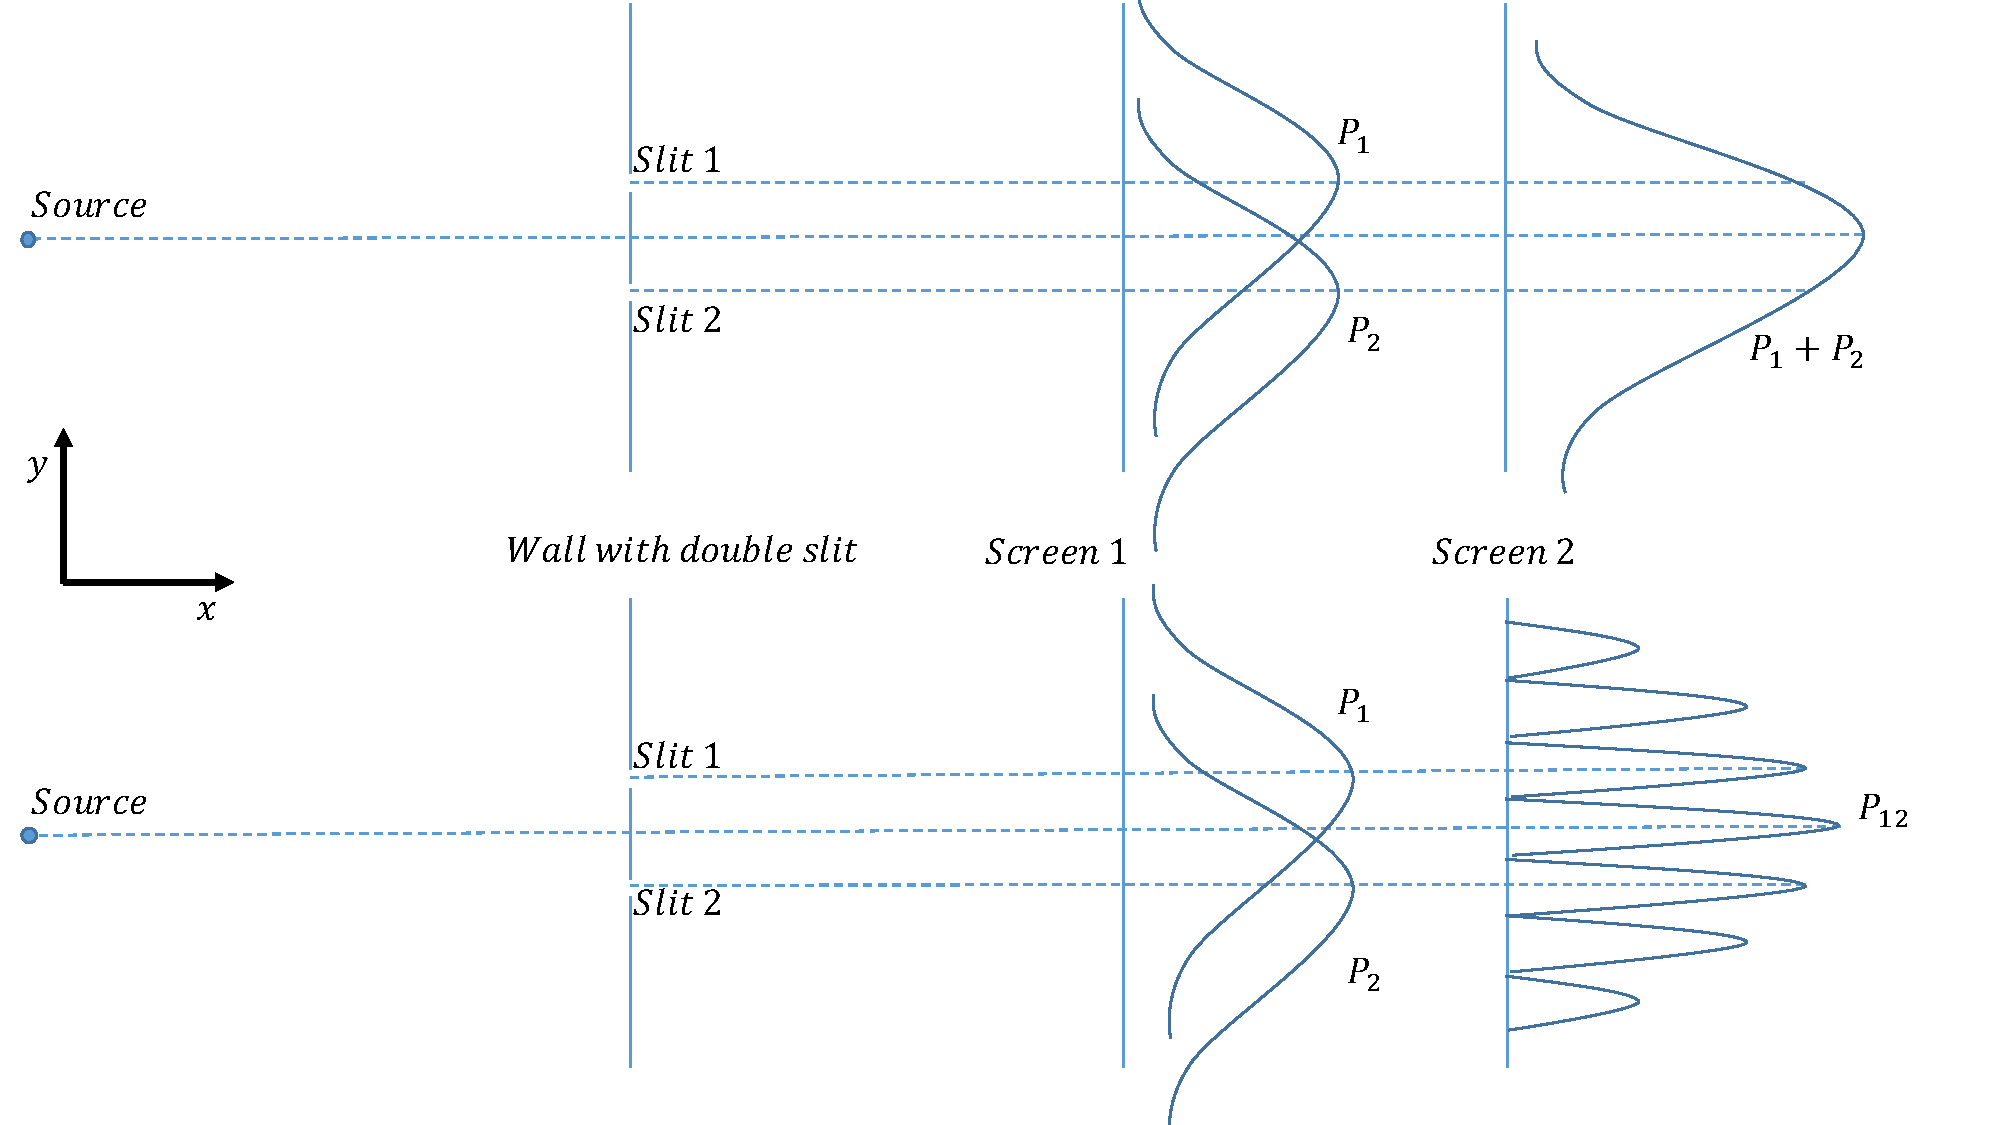
\includegraphics[scale = 0.5]{DSe.pdf}
\caption{Schematic of the double slit experiment. The diagram shows two different scenarios. The top figure shows the behaviour one would expect of classical particles going through one slit or the other. The bottom figure shows the behaviour of classical waves creating an interference patter. Screen one shows the signal that one would see in each scenario (i.e classical particles or waves) if only one slit was open. If slit 1 was open we would see $P_1$ and see on. Screen 2 shows the signal we see if both the silts are open in each scenario.}
\label{fig-doubleslit}
\end{center}
\end{figure}

This standard explanation works because we assume the particle is the only quantum-mechanical system here, and it can be describe by a pure state, $|\phi\rangle_{\rm particle} = |\phi_1\rangle + |\phi_2\rangle$.
But if quantum mechanics is correct, this particle is not the only thing to be described by a wavefunction. 
For example, we can also describe the double-slit by its wavefunction $|\psi\rangle_{\rm ds}$. The total wavefunction of the combined system can be in a pure state,
\begin{equation}
|\Psi\rangle_{\rm combined} = |\psi_1\rangle_{\rm ds}|\phi_1\rangle_{\rm particle} 
+ |\psi_2\rangle_{\rm ds}|\phi_2\rangle_{\rm particle} ~,
\end{equation}
but either subsystem does not have to be pure.

When the two double-slit states are almost indistinguishable,
\begin{equation}
\langle\psi_1|\psi_2\rangle\langle\psi_2|\psi_1\rangle \approx 1~,
\label{eq-pure}
\end{equation}
then the combined system factorizes,
\begin{equation}
|\Psi\rangle_{\rm combined} \approx |\psi_1\rangle_{\rm ds}
\left(|\phi_1\rangle_{\rm particle} + |\phi_2\rangle_{\rm particle}\right) ~.
\end{equation}
The particle subsystem indeed stays as a pure state and there will be an interference pattern.

On the other hand, if the two double-slit states are distinguishable,
\begin{equation}
\langle\psi_1|\psi_2\rangle\langle\psi_2|\psi_1\rangle \ll 1~,
\label{eq-mixed}
\end{equation}
that means the interaction entangled the two systems. The particle subsystem becomes a mixed state,
\begin{equation}
\rho_{\rm particle} = {\rm Tr}_{\rm ds}|\Psi\rangle\langle\Psi| \approx
|\phi_1\rangle\langle\phi_1| + |\phi_2\rangle\langle\phi_2|~,
\end{equation}
and there will be no interference pattern.

Whether the double-slit states are given by Eq.~(\ref{eq-pure}) or (\ref{eq-mixed}) seems to require the knowledge about the actual quantum-mechanical interacton between the particles and the double-slit, which is unavailable in practice.
Feynman pushed the above analysis further to overcome such problem.
He pointed out that even if we try to keep the interaction minimal, there will be one inevitable interaction that makes $|\psi_1\rangle$ and $|\psi_2\rangle$ different.
That is because when a particle reaches some place on the screen, its $y$-momentum must be different depending on which slit it passed through.
\begin{equation}
\Delta p_y^{\rm particle} \equiv 
|\langle\phi_1|p_y|\phi_1\rangle - \langle\phi_2|p_y|\phi_2\rangle| 
\approx p_x \frac{s}{L}~,
\end{equation}
where $p_x$ is the $x$ momentum of the particles, $s$ is the separation between the two slits, and $L$ is the distance to the screen. 
This means two different values of recoil momentum on the double-slit,
\begin{equation}
\Delta p_y^{\rm ds} = \Delta p_y^{\rm particle} \approx p_x \frac{s}{L}~.
\label{eq-dpds}
\end{equation}
The uncertainty principle sets a limit on how well we can measure this difference. Namely, we need a large uncertainty in the position to measure a small change in momentum. Setting $\hbar$ to 1, we can say that when the momentum difference is too small to be measured,
\begin{equation}
\Delta p_y^{\rm ds} < 1/\Delta y^{\rm ds}~,
\label{eq-standard}
\end{equation} 
then Eq.~(\ref{eq-pure}) is true and the two states are indistinguishable. 
Otherwise Eq.~(\ref{eq-mixed}) is true and the two states are distinguishable.

The key point is that there is an alternative way to appreciate Eq.~(\ref{eq-standard}) {\it without} thinking about the quantum mechanics of the double-slit. 
First of all, the interference pattern has a fringe width of  
\begin{equation}
w = L\frac{\lambda}{s}~,
\end{equation}
where $\lambda = p_x^{-1}$ is the de Broglie wavelength of the particle. This is the separation of bright/dark lines in the $y$ direction with a fixed reference point at the $y$ position of the double-slit. Thus the uncertainty in the $y$ position must be smaller than this value, so the interference pattern is not totally blurred.
\begin{equation}
\Delta y^{\rm ds} < w = \frac{L}{p_xs}~.
\label{eq-stdcls}
\end{equation}
This is exactly the same condition as in Eq.~(\ref{eq-standard}).

We should emphasize the key value of this result. 
We can treat both the position uncertainty $\Delta y^{\rm ds}$ and the interference fringe width $w$ as classical quantities. Eq.~(\ref{eq-stdcls}) is then a purely classical calculation to compare these two quantities, which tells us whether a classical wave pattern (the intereference pattern) loses coherence. 
If we only take its face value, it seems to be only a practical obstacle of measuring the interference pattern. 
One might argue that the underlying subsystem unitarity is still valid, just difficult to measure. 

What Feynman showed by this example is that Eq.~(\ref{eq-stdcls}) tells us exactly the same thing as Eq.~(\ref{eq-standard}). 
The later {\bf is} directly about quantum mechanics and shows how the subsystem unitarity can fail. 
Thus an apparently classical calculation can tell us something about the hidden quantum-mechanical nature of the interaction between the double-slit and the particle passing through it. 
In this example, it tells us whether the particles get entangled with the double-slit and loses its subsystem unitarity. 

One might object that the Eq.~(\ref{eq-stdcls}) is not entirely classical, since the value of $\Delta y^{\rm ds}$ has to originate from the unknown quantum mechanics of the double-slit. 
This is a valid concern, and it actually shows another strength of Eq.~(\ref{eq-stdcls}). 
Indeed we do not know the value of $\Delta y^{\rm ds}$ just from classical physics, but it is very reasonable to assume that it is intrinsic to the double-slit. 
Namely, its value should be fixed if we move the screen further away. Eq.~(\ref{eq-stdcls}) shows that with a fixed $\Delta y^{\rm ds}$, we can always make $L$ large enough to satisfy this condition. 
Thus, at least at the level of gedanken experiment, one can always arrange a situation that the interference pattern is visible, thus the subsystem unitarity is valid.

\section{Analogy in Quantum Field Theory}
\label{sec-QFT}

The double-slit interference is an example that both the classical coherence and quantum unitarity can be calculated explicitly and show that they follow the same condition.
Here, we advocate that such a relation is actually a general rule.
{\it Classical coherence, instead of thinking of it as a practicality of measurements, should be treated as a prerequisit to quantum unitarity.} 
Thus when classical coherence fails, not only have we no practical measurements to confirm the purity of the subsystem wavefunction, such wavefunctions {\it actually did not evolve unitarily.}
Whatever effect responsible for a classical uncertainty large enough to disrupt classical coherence must have also interacted with the subsystem quantum-mechanically and became entangled with it.

For quantum field theory in a curved spacetime, we always assume that the quantum field is a subsystem that never entangles with the geometry, thus remains unitary.
Since we do not know quantum gravity/geometry, we cannot directly check this assumption by an actual calculation of entanglement.
However, we can always check classical coherence, and by this rule we advocate, the answer directly proves/disproves subsystem unitarity.

If we go back to the basic of quantum field theory, there is a natural generalization of this new rule. 
As shown in Fig.\ref{fig-QFT}, QFT starts from solving a classical mode function, then quantizing its amplitude into a quantum state. 
Any method to measure such quantum state assumes the knowledge of the classical mode function. 
If the geometric uncertainty leads to an order one change in the classical mode function, then there is no practical way to reliably measure its quantum state. 
We advocate that this is not only a practicality about measuring the quantum state, but it directly tells us that the quantum state loses its unitarity. 
Just like in Feynman's example where the uncertainty of the double-slit guarantees its entanglement with the particles, whatever effect that leads to the geometric uncertainty here must entangle with the quantum state of this mode. 
Without a theory of quantum geometry, we cannot describe how that happens. 
But through a classical calculation, we can determine whether it has happened or not.

\begin{figure}[h!]
\begin{center}.
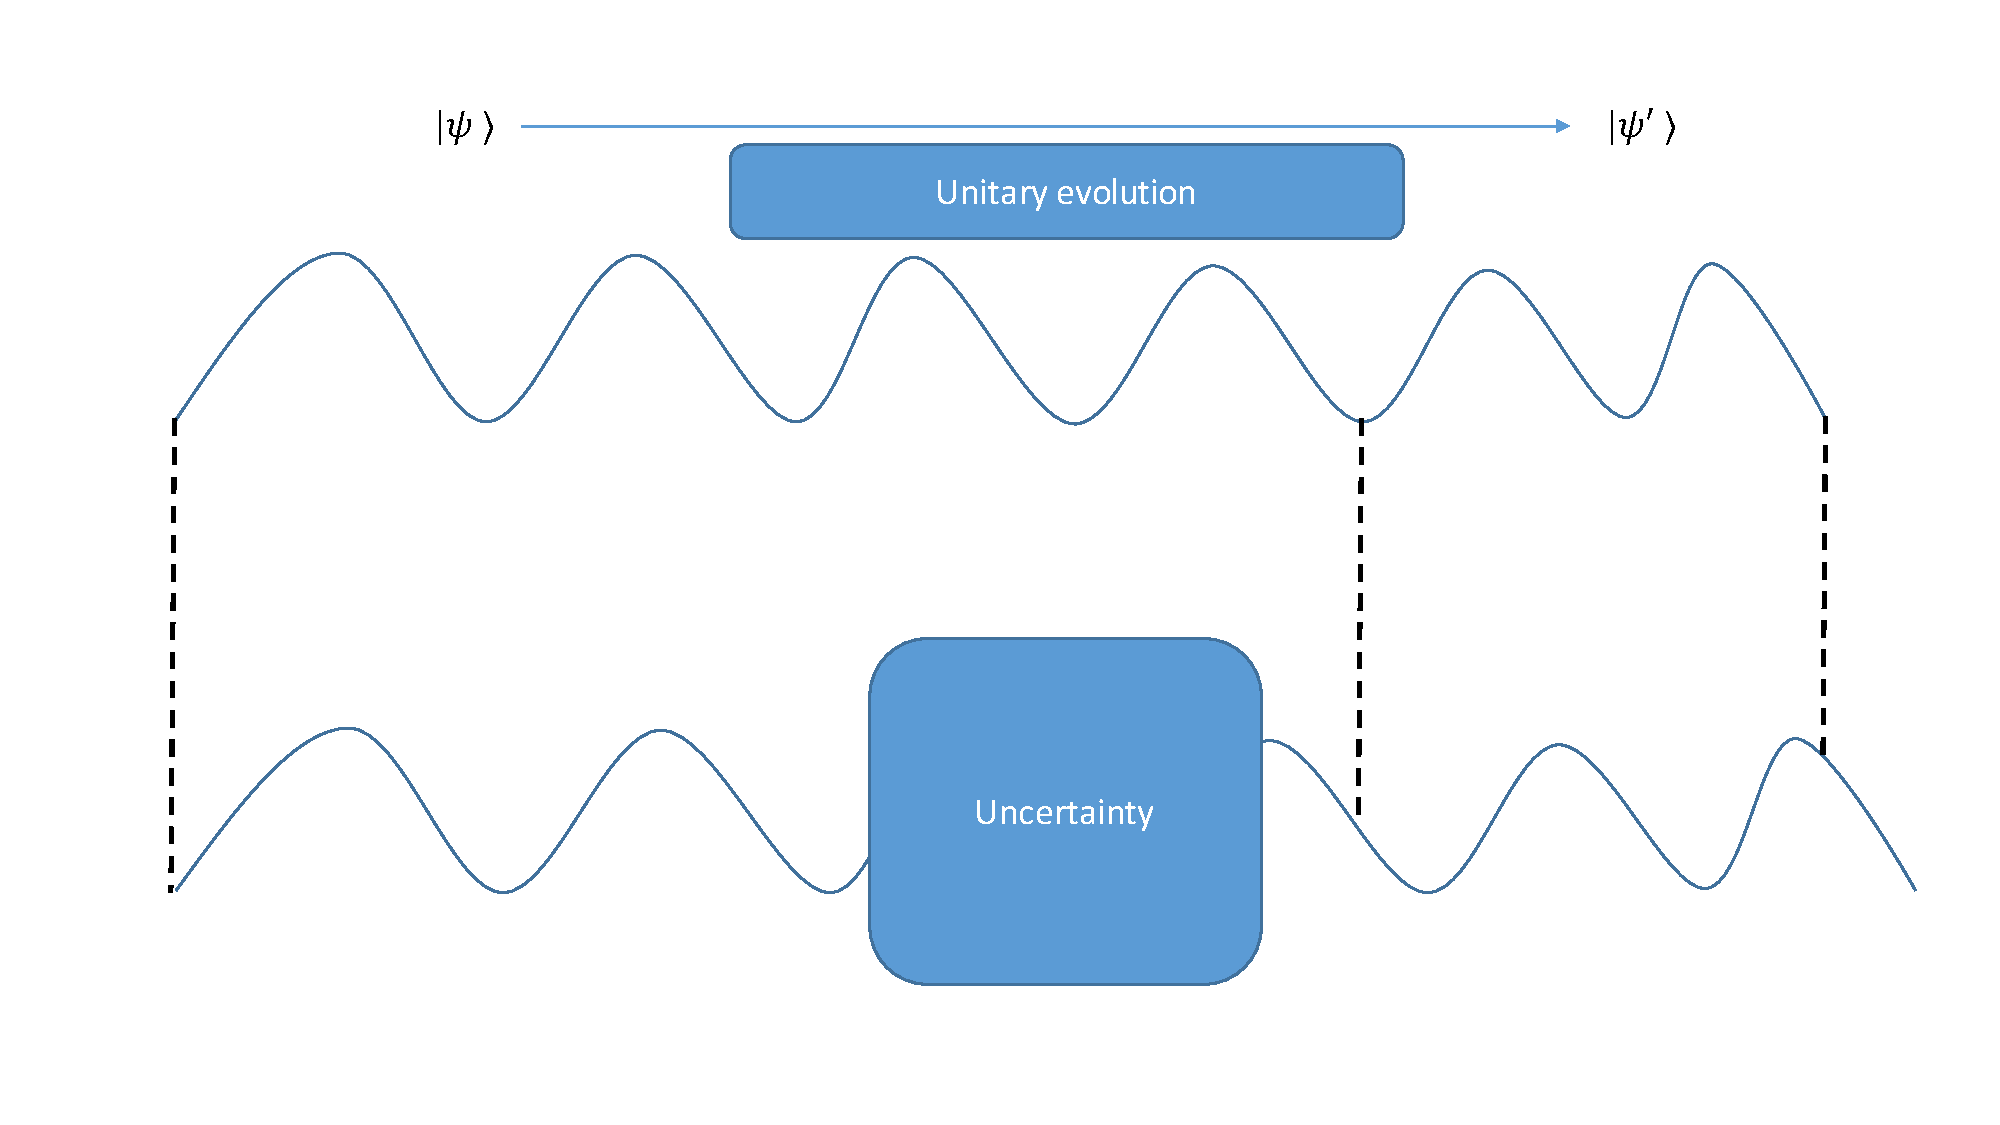
\includegraphics[scale = 0.5]{bh_coherence.pdf}
\caption{Schematic showing the rule we advocate; as classical coherence fails, we loose quantum unitarity.}
\label{fig-QFT}
\end{center}
\end{figure}

While such generalization to QFT seems straightforward in theory, there are a few subtleties in practice.
In the double-slit experiment, the position uncertainty of the double-slit was the only obvious uncertainty of the background that we need to keep track of.
It is also the reasonable thing to hold fixed while moving the projection screen away.
In QFT, the background is the entire geometry, and there are infinitely many ways a geometry can be uncertain.
For a full analogy to Feynman's analysis, not only we need to parametrize those uncertainties, we also need to choose the appropriate combination to hold fixed as we take a similar limit.
At this moment, we do not have a general formalism to setup such self-consistency check that can be applied to any general geometry. 
In Sec.\ref{sec-BlackHole}, we propose a specific way to apply such self-consistency check to the propagation of Hawking quanta.
In addition to gaining insights into the information paradox, we hope to learn some lessons to inspire a more general formalism of such self-consistency check.

QFT theorists might think that a more direct self-consistency check is feasible.
Instead of parametrizing a classical geometric uncertainty, one can treat deviations from the background geometry as a field and quantize it as any other fields.
Then a standard QFT calculation of scattering with this new field (graviton) should capture all interactions with the geometry, and a small scattering amplitude should guarantee that the interaction is suppressed. 
The concern for such method is that IR issues for these scattering calculations cannot be unambiguously regulated like in global Minkowski space.
Since soft gravitons lead to real physical changes in the geometry that can be seen in memory effects \cite{Wei65,HeLys14}, an IR ambiguity signals our ignorance on how these geometric changes enter QFT.
Thus a direct graviton scattering calculation cannot be the full extend of a self-consistency check, and it is reasonable for our method to give extra constraints on the reliability of local QFT.

\section{Hawking quanta propagation}
\label{sec-BlackHole}

The usual treatment of how a near-horizon mode becomes an asymptotic Hawking quantum is also following a fixed-background assumption.
The background is the Schwarzschild geometry.
\begin{equation}
ds^2 = -\left(1-\frac{2M}{r}\right)dt^2 + \frac{dr^2}{1-\frac{2M}{r}} + r^2d\Omega_2^2~.
\end{equation}
When one applies local quantum field theory to describe a field on this fixed background, the result is by-definition unitary, but that is not necessary a physical fact. 
Given how little we understand quantum gravity, a classical self-consistency check as we described in the previous section is a reasonable thing to do.

\subsection{Setup and summary}

\begin{itemize}
\item {\bf Classical coherence by tracking geodesics.} The classical mode of a massless field basically has its peaks and nodes following null geodesics.
Thus, instead of actually solving the mode function, we can perform a much simpler calculation to track geodesics.
We start with two out-going null geodesics with the separation of one period of such mode near the horizon, and then we calculate the change in their separations at spatial infinity.
If this change is comparable to the wavelength, then the mode function of this wavelength loses classical coherence.
\item {\bf The background and the uncertainty.} The classical background in this case is the Schwarzschild geometry, which can be written as the metric $g_{\mu\nu}$. 
A classical uncertainty can be expressed as deviation from such metric, $\Delta g_{\mu\nu}$. 
There are two major challenges here.
\begin{enumerate}
\item There are many more variables than the double-slit experiment. 
We consider only one particular form of $\Delta g_{\mu\nu}$ in this paper---back-reactions from the presence of extra matter of zero total energy. 
It is simple to calculate and reflects the physcial intuition of vacuum pair fluctuation.
\item The value of $\Delta g_{\mu\nu}$ is gauge dependent. 
By relating it to the presence of extra matter, we can express it as a gauge-invariant local quantity, which is the natural thing to hold fixed in our analysis.
\end{enumerate}
Note that if we were reporting a positive result, that such uncertainty upholds unitarity, then one should question the validaty of learning a general lesson from a special example. However, we will show that this particular form of $\Delta g_{\mu\nu}$ is already sufficient to question unitarity, and we did not choose this form to specifically do that. Thus our limited analysis is sufficient to raise a reasonable doubt to the classical-background approximation.
\item {\bf Renormalization.} It is well-known that na\"ive applications of QFT often suffer from UV/IR divergences.
In our case, we will see that even in Minkowski space, geometric uncertainty already leads to a finite change between the two null geodesics.
We will simply ``renormalize'' that away by saying that if the black hole case leads to a similar change, it should not be taken as a serious problem.
Our surprising result is that in the black hole case, we get an infinitely larger change, which is difficult to blame on renormalization.
\end{itemize}

More concretely, our setup is shown in Fig.\ref{fig-setup}. 
We start by choosing two points at some $r_0\gg M$ with a $\delta t_0\sim M$ coordinate time separation between them.
This represents one wavelength of the mode function of an asymptotic Hawking quantum.
We then back-track two null geodesics from these two points back to two points near the horizon, at $r_A$ with $(r_A-2M)\ll 2M$.
Now their separation represents one wavelength of a near-horizon mode, which would have propagated to the asymptotic mode if there were no geometric uncertainty. 
We then introduce introduce a geometric uncertainty as two shells of zero total ADM mass. 
Therefore, both the near horizon and the asymptotic regions are not affected by such uncertainty.
Only the process of propagation is affected.
With the same two starting points near the horizon. we calculate the separation $\bar{\delta t_0}$ of the two null geodesics when they arrive at $r_0$, and compare it with $\delta t_0$.

\begin{figure}[tb]
\begin{center}
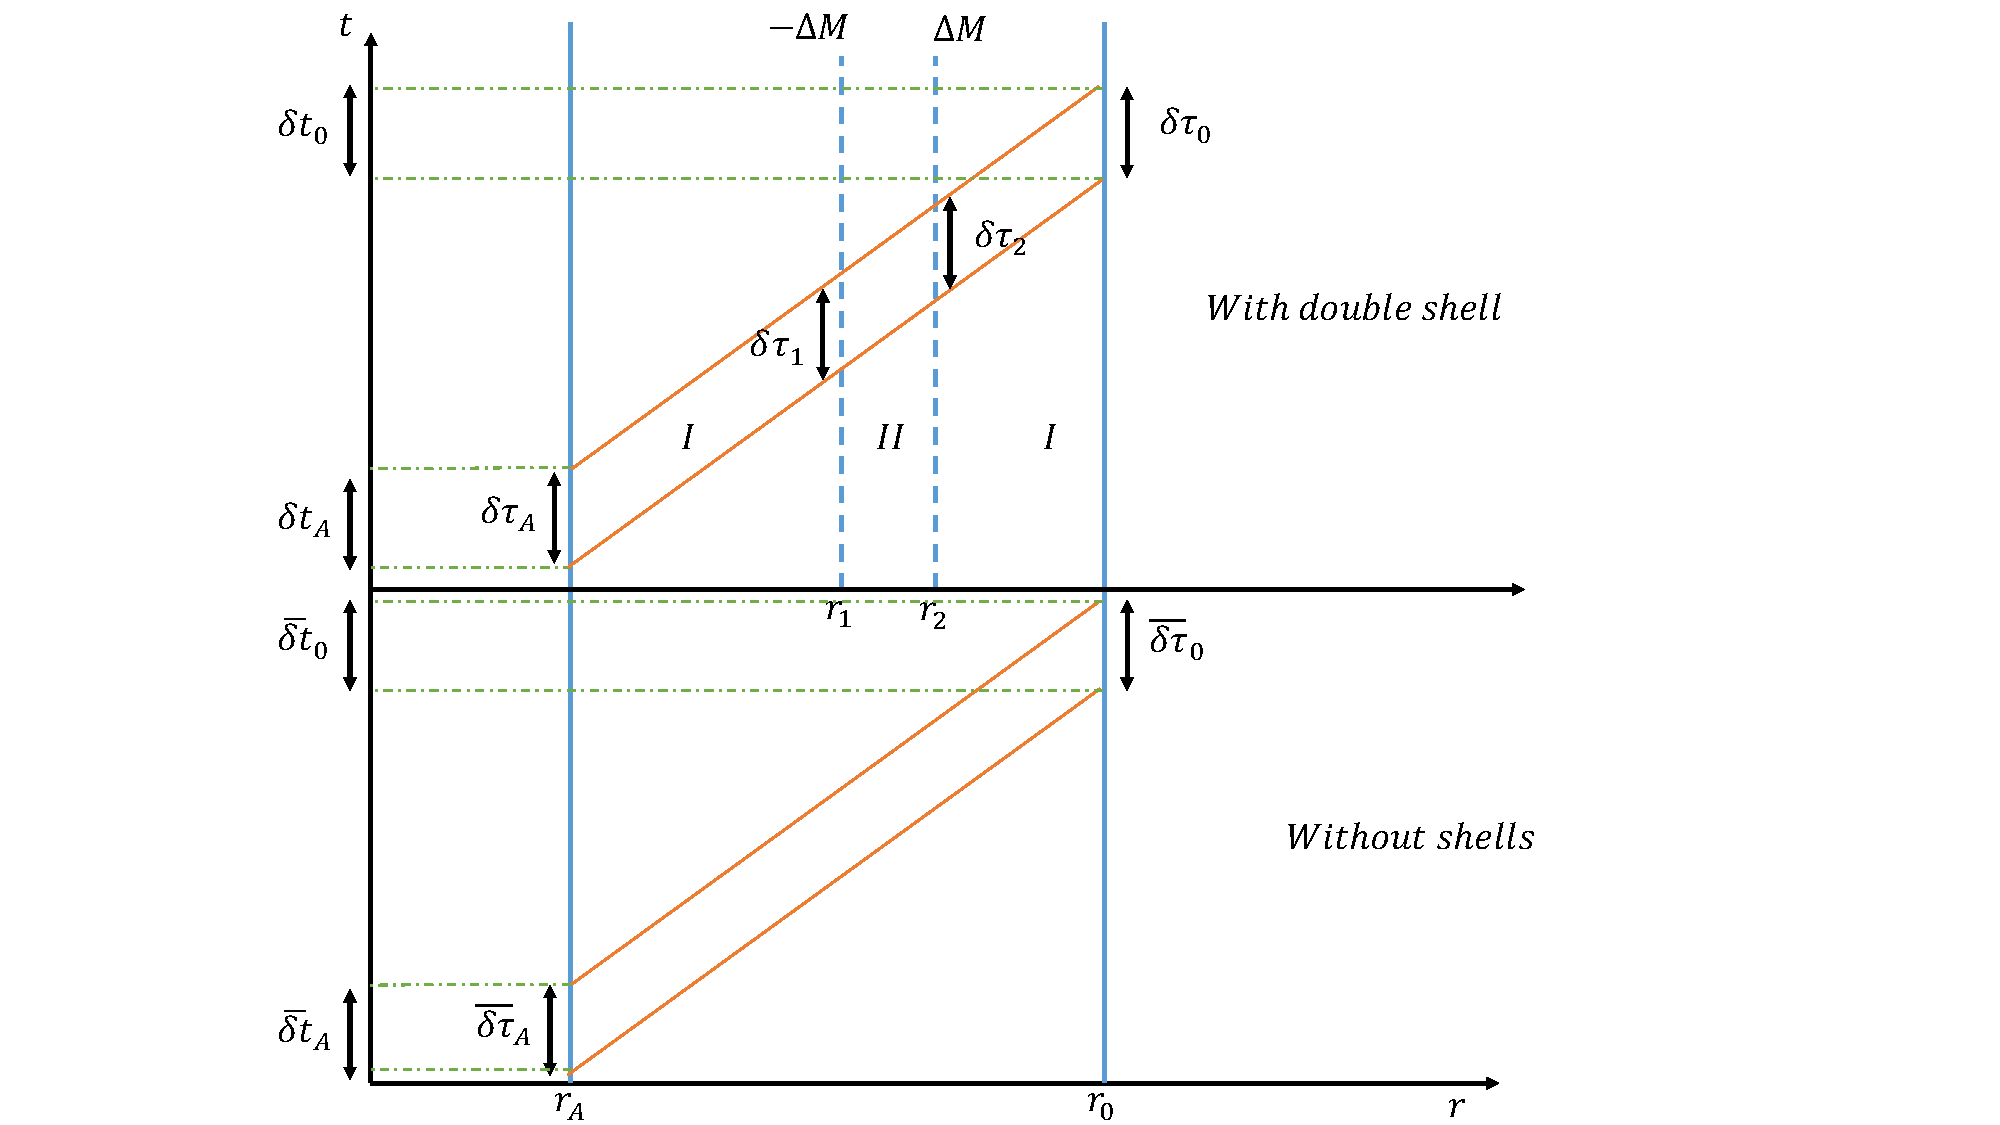
\includegraphics[scale = 0.6]{Propertime.pdf}
\caption{The two parts of this diagrams describe two different scenarios. The trajectories of the photon are the lines in orange. The trajectory of the observer and the position from which the photons are emitted are represented by solid blue lines. The bottom part is a general case of two Hawking photons coming from a distance $r_A$ from the black hole of mass $M$ and arriving at an observer who is at a distance of $r_0$. The top part shows two Hawking photons coming from the same distance $r_A$ from a black hole of mass $M$. Instead of the photons freely propagating through to an observer at $r_0$, they have to cross two shells, represented by blue dotted line, of equal and opposite mass $-\Delta M, \Delta M$ at $r_{1}, r_{2}$ respectively. The regions $I$ represent a metric with mass $M$ and region $II$ represents a metric with mass $M-\Delta M$.}
\label{fig-setup}
\end{center}
\end{figure}

After some formal calculations in the {\bf Appendix}, we arrive at this simple expression:
\begin{equation}
\frac{\delta t_0 - \bar{\delta t_0}}{\delta t_0} = 
\left(\sqrt{\frac{r_2-2M}{r_1-2M}}\sqrt{\frac{r_1-2(M-\Delta M)}{r_2-2(M-\Delta M)}}-1\right)~,
\label{eq-result}
\end{equation}
where $r_1$ is the location of the inner shell, $r_2$ is the location of the outer shell, and $\pm\Delta M$ are their individual ADM masses.

\subsection{Physical interpretation}

As the first step, we set $M=0$ in Eq.~(\ref{eq-result}) to study its meaning in Minkowski space. Assuming that $|r_1-r_2| \equiv \Delta r \ll r_1$ and $\Delta M \ll r_1$, the leading order result becomes
\begin{equation}
\frac{\delta t_0 - \bar{\delta t_0}}{\delta t_0} \approx - \frac{\Delta M}{r_1^2} \Delta r 
\equiv \sigma \Delta r~.
\label{eq-Mink}
\end{equation}
This seems to be a reasonable answer. 
First of all, it is quite unlikely that the entire shell of mass $\Delta M$ fluctuates out of vacuum.
It is reasonable that any change to the null geodesics is about a local energy density of the particular piece of shell they happen to pass through.
Secondly, this result is gauge invariant. For an observer at rest, $\sigma$ is the local energy density and $\Delta r$ is the proper distance. 
For a boosted observer, $\sigma$ increases by a boost factor while $\Delta r$ contracts by the same factor.
We take it as a good sign that other forms of geometric uncertainty can also be parametrize by a similar, gauge invariant quantity.

The na\"ive interpretation of Eq.~(\ref{eq-Mink}) is that even in Minkowski space, geometric uncertainty can potentially decohere classical mode functions.
By our definition, that poses some threat to QFT in Minkowski space.
We are going to assume that unitarity in QFT is fine in Minkowski space, effectively ``renormalize away'' the effect of Eq.~(\ref{eq-Mink}).
One can imagine a simple subtraction by a counter term.
Or alternatively, since the actual value of $(\sigma\Delta r)$ is unknown, we assume that it is small enough to not cause any concern.

Next we study Eq.~(\ref{eq-result}) with an actual black hole. 
When the double-shell is very far away from the black hole, $r_1\gg M$, it agrees with Eq.~(\ref{eq-Mink}) as expected. 
The interesting thing here is that when this pair of geodesics originate near the horizon, the double-shell could also be somewhere near the horizon. 
In that limit, Eq.~(\ref{eq-result}) can be approximated by
\begin{equation}
\frac{\delta t_0 - \bar{\delta t_0}}{\delta t_0} \approx
- \sigma \Delta l \left(\frac{2M}{l}\right)^2~, \ \ \ \ {\rm \bf XXX \ check \ coefficients}
\label{eq-NearHorizon}
\end{equation}
where $l$ is the proper distance between $r_1$ and the horizon and $\Delta l$ is the proper distance between the two shells. 
We can see that in addition to the same gauge-invariant quantity in Minkowski space
\footnote{In Minkowski space, the radial coordinate is the proper distance, $\Delta r=\Delta l$.}, 
there is an extra factor of $(2M/l)^2$ which diverges as the shell approaches the horizon.

The small $l$ limit may not be the best way to appreciate how Eq.~(\ref{eq-NearHorizon}) poses a threat to QFT. 
After all, we do not expect QFT to hold for arbitrarily small distance anyway. 
The best way to understand Eq.~(\ref{eq-NearHorizon}) is to fix $l$ at some scale that much longer than any scale that we expect UV problems. 
By conventional knowledge, the effect of gravity near horizon gets arbitrarily weak as the black hole becomes large. 
However, the problem caused by Eq.~(\ref{eq-NearHorizon}) grows larger as the black hole becomes larger, and diverges in the large black hole limit.
Since the large black hole limit is supposed to be the best case scenario for information paradox, such a diverging uncertainty to decohere classical waves causes a strong doubt on the subsystem unitarity assumption in QFT.


\section{Discussion}
\label{sec-dis}

\subsection{The self-consistency check of local QFT}

In this paper, we proposed a self-consistency check of local QFT in curved spacetime geometries.
We have shown that the near-horizon geometry of a Schwarzschild black hole seems to fail such a check.
As explained in Sec.\ref{sec-BlackHole}, the consistency requires us to parametrize the uncertainty in the classical geometry.
We have chosen a particular form of uncertainty in our explicit calculation.
Our result is gauge invariant and makes physical sense, but there might be a more general way to parametrize such uncertainty to make our approach even more general.
It is also interesting to apply the same check to other geometries, especially other types of horizons.

We should emphasize that our check does not invalidate QFT all together.
We simply suggest that the QFT degrees of freedom lose their subsystem unitarity.
In the double-slit experiment, with or without the interference pattern, the total number of particles that passes through the double-slit is not affected, and the expectation value of the particle location remains in the center.
The point is that we can always find a pair of pure and mixed density matrices which give identical expectation values to many observables.
It is not unexpected that the only affected observable is the one explicitly checking unitarity.
Thus we can still rely on QFT to calculate the values of other observables.

Many existing results of QFT in curved/dynamical geometries are about particle numbers, such as the particle-production calculation following a Bogoliugov transformation. 
As an example, one can easily see that
\begin{equation}
\rho_{\rm pure} = \left(\sum_n a_n|n\rangle\right)
\left(\sum_n \langle n| a_n^*\right)
\end{equation}
and
\begin{equation}
\rho_{\rm mixed} = \sum_n |a_n|^2 |n\rangle\langle n|
\end{equation}
give the same particle number. 
Thus there is no general crisis if we admit that local QFT sometimes loses subsystem unitarity. 

As far as we know, an observable that explicitly checks the subsystem unitarity of local QFT is the cosmological Bell inequality \cite{Mal15}. 
One can apply our self-consistency check to such a model and update the prediction of whether a violation of Bell inequality is actually expected.


\subsection{The information-transfer puzzle}

Showing the lack of unitarity in the propagation of Hawking quanta does not resolve all the problems. 
Usually, one pictures a nonunitarity process as losing information. 
In the context of black hole information, a Hawking quantum actually has to {\it recover} information. 
A near-horizon mode starts from a maximally mixed (thermal) state with no information, since its partner is the interior mode that never comes out of the horizon. 
After the nonunitarity propagation to become an asymptotic Hawking quantum, it has to carry information to purify the rest of the Hawking radiation there.

Since unitarity is lost to the local geometric uncertainty, what restores information must be the interaction with the local geometry. 
An abstract realization of this information-recovery process is recently demonstrated in \cite{OsuPag16}. 
In order for local geometry to give this information to the Hawking quanta, it must first carry such information.
If was first suggested that superpositions of different classical geometries can store such information \cite{NomVar12}.
In the conventional picture, classical geometries are determined by only a few parameters such as the location and size of the black hole.
Thus the major objection to such picture is that the superpositons of classical geometries do not form a large enough Hilbert space to hold the required information.
Recently, it was realized that there are actually a much larger number of classical geometries differed by their soft hairs \cite{HawPer16}.
A simple counting suggested that the size of Hilbert space seems no longer the problem, so one should persue this line of thoughts even further.

Classically, soft hairs manifest as memory effects that alters the distances between geodesics, which is very similar to the effect of geometric uncertainty as we showed in this paper.
Based on this picture, one may try to quantize the soft hairs and build a toy model that involves quantum interaction, therefore entanglement, between the soft hairs and the usual QFT modes.
That would provide a complete picture that the loss of subsystem unitarity is really just entanglement with another subsystem which was originally (and illegitimately, as we argued) assumed as the classical background.


\appendix


\section{Calculation}

A black hole of mass $M$ defines a Schwarzschild geometry for the spacetime with the following metric 

\begin{equation}
	ds^2 = - \left( 1 -\frac{2M}{r} \right) dt^2 + \left( 1 - \frac{2M}{r} \right)^{-1} dr^2 + r^2 d \Omega_2^2	\label{1}
\end{equation}

where we are working with units in which $G = c = 1$. We know there will be a flux of particles appearing from the horizon of the black hole \cite{Haw74}. Take some coordinate time interval, $\delta \bar{t_e}$, (which will have some corresponding proper time interval $\delta \bar{\tau_e}$) between two consecutive particles being emitted from the same position above the horizon of the black hole. An observer far away will see these particles arrive with some coordinate time interval $\delta \bar{t_0}$. We can follow the trajectory of the particles (assuming they are relativistic) from the position they are emitted, $r_e$, to the observer at $r_0$ by setting $ds = 0$ in Eq (\ref{1}). By confining the motion to be only in the radial direction, i.e $d \Omega_2 = 0$, we get the following geodesic equation

\begin{equation}
	\bar{t_e}^{(1)} - \bar{t_0}^{(1)} = \bar{r_0} - \bar{r_e} + 2M \ln \left( \frac{\bar{r_0} - 2M}{\bar{r_e} - 2M}  \right)	\label{3}
\end{equation}

where the superscript represents particle $1$. An analogous geodesic equation is given for particle 2. 

\begin{equation}
	\bar{t_e}^{(2)} - \bar{t_0}^{(2)} = \bar{r_0} - \bar{r_e} + 2M \ln \left( \frac{\bar{r_0} - 2M}{\bar{r_e} - 2M}  \right).	\label{4}
\end{equation}

Since the right hand side of Eq (\ref{3}) and (\ref{4}) is the same, we see that

\begin{equation}
	\bar{t_0}^{(2)} - \bar{t_0}^{(1)} = \bar{t_e}^{(2)} - \bar{t_e}^{(1)} \Rightarrow \delta \bar{t_0} = \delta \bar{t_e}.
\end{equation}

Therefore the coordinate time interval when the particles are emitted remains the same when it is observed at distance $r_0$ as is shown in the bottom part of figure \ref{fig-setup}.

%We can convert $\delta\bar{t_0}$ to proper time
%
%\begin{equation}
%	\delta \bar{\tau_0} = \left( 1 -\frac{2M}{r_0} \right)^\frac{1}{2} \delta \bar{t_0}
%\end{equation}
%
%and in the limit that the observer is very far away $\delta \bar{\tau_0} \approx \delta \bar{t_0}$. 

\subsubsection{Perturbed spacetime - double shell}

Now we introduce two shells of matter with equal and opposite ADM mass, $-\Delta M$ and $\Delta M$ where $|\Delta M|<<M$, at a distance of $r_1$ and $r_2$ respectively as shown in the top part of figure \ref{fig-setup}. We model these shells as infinitesimally thin and therefore use the Israel Junction Conditions (IJC) \cite{Isr66} with a delta function shell to analyze the effects of the shells. In this case the particle's move through two different spacetime regions. Region $I$ is defined by the black hole of mass $M$ and region $II$ is defined by a Schwarzschild metric of mass $M-\Delta M$ as shown in the top part of figure \ref{fig-setup}.
\\
\\
As explained in the previous section, the proper time interval between two particles emitted at $r_e$, $\delta t_e$, is the same as the coordinate time interval at $r_1$, $\delta t_1$. Now we need to find the corresponding coordinate time interval in region $II$, $\delta \hat{t}_1$ (in general we will use hats on top of quantities that are evaluated in region $II$). To do this we simply note that the corresponding proper time at $r_1$, $\delta \tau_1$ must be the same in both regions of spacetime - this is a simple consequence of the IJC. The coordinate time intervals at $r_1$, in the two different regions, are therefore related by

\begin{equation}
	\delta t_1 = \delta t_0 = \left( \frac{1 - \frac{2(M - \Delta M)}{r_1}}{1 - \frac{2M}{r_1}} \right)^\frac{1}{2} \delta \hat{t}_1.
\end{equation}

We can propagate the particles through region $II$ from $r_1$ to $r_2$ and we know $\delta \hat{t}_1 = \delta \hat{t}_2$. From the fact that the proper time corresponding to the coordinate time intervals will be the same, we can relate $\delta \hat{t}_2$ back to $\delta t_2$ in region $I$, 

\begin{equation}
	\delta \hat{t}_2 = \delta \hat{t}_1= \left( \frac{1 - \frac{2M}{r_2}}{1 - \frac{2(M- \Delta M)}{r_2}} \right) \delta t_2.	\label{7}
\end{equation}

Since $\delta t_2$ is equal to the time interval observed by the observer at $r_0$, $\delta t_0$, we can find the proper time observed by the observer, $\delta \tau_0  = \delta t_e \left( \left( \frac{r_2 - 2M}{r_1 - 2M} \right) \left( \frac{r_1 - 2(M-\Delta M)}{r_2 - 2(M - \Delta M)} \right) \right)^\frac{1}{2}$. Where we have dropped the $\left( 1 - \frac{2M}{r_0} \right)^\frac{1}{2}$ term since we assume the observer is very far away. $\delta t_e = \delta \bar{\tau_0}$ when the observer is far away therefore we can define a dimensionless quantity that quantifies the change in proper time intervals for consecutive photons in perturbed spacetime case and the unperturbed case, 

\begin{equation}
	 \frac{\delta \tau_0 - \delta \bar{\tau_0}}{\delta \bar{\tau_0}} = \left( \left( \frac{r_2 - 2M}{r_1 - 2M} \right)^\frac{1}{2} \left( \frac{r_1 - 2(M-\Delta M)}{r_2 - 2(M-\Delta M)} \right)^\frac{1}{2} - 1\right).	\label{10}
\end{equation}

This expression is exact in the limit that the observer is far away. By expressing the distances from the horizon as, $r_1  =  2M + \epsilon,  r_2  =  2M + \epsilon + \delta \epsilon$, we can write Eq (\ref{10}) as

\begin{equation}
	\frac{\delta t_0 - \bar{\delta t_0}}{\delta t_0} = \left( \left( \frac{\epsilon + \delta \epsilon}{\epsilon} \right)^\frac{1}{2} \left( \frac{\epsilon + 2 \Delta M}{\epsilon + \delta \epsilon + 2\Delta M} \right)^\frac{1}{2} - 1\right). \label{12}
\end{equation}

This shows that when there are no shells, $\Delta M = 0$, there is no change in proper time intervals which is what one would expect. More interestingly we see that there is no $M$ dependence in this equation. This suggests the effect is present in flat space as well. One may interpret this effect as being a phase shift between the photons as the travel through two different gravitational potential wells. Before jumping to any conclusions, however, we should convert the coordinate quantities in Eq (\ref{12}) into physical quantities. 
	
%
%where $\epsilon<<2M, \ \epsilon << \epsilon$. To leading order in small quantities Eq (\ref{10}) becomes, 
%
%\begin{equation}
%	\frac{\delta \tau_0 - \delta \bar{\tau_0}}{\delta \bar{\tau_0}} = - \frac{\Delta M \epsilon}{\epsilon^2}.	\label{11}
%\end{equation}

\subsection{Defining local quantities}

\subsubsection{Energy of shell}

There is a natural choice of what physical quantity we should use to replace $\Delta M$ with and that is the $tt$ component of the surface stress energy tensor, $S_{ab}$, of the shell as computed by the IJC

\begin{equation}
	S^a_b =  [K^a_b] - [K]h^a_b
\end{equation}

where $K_{ab}$ is the extrinsic curvature corresponding to the induced metric we are using, $K = K_{ab} h^{ab}$ is the trace of the extrinsic curvature taken with respect to the induced metric and the notation of square brackets represents the difference in a quantity in two different induced metrics. 
%
%We can define the induced metrics for constant $r$ values; for region $I$ it is 
%
%\begin{equation}
%	ds_{3M}^2 = - \left( 1 - \frac{2M}{r} \right)^{-1} dt^2 + r^2 d \Omega_2^2.	\label{13}
%\end{equation}
%
%Analogously we have the metric corresponding to mass $M' = M- \Delta M$ in region $II$
%
%\begin{equation}
%	ds_{3M'}^2 = - \left( 1 - \frac{2M'}{r} \right)^{-1} dt'^2 + r^2 d \Omega_2^2.	\label{14}
%\end{equation}
%
%We could rewrite Eq (\ref{13}) and (\ref{14}) in Gaussian normal coordinates (where the coefficient in front of the time component is 1), however the first order junction condition is that the induced metric on both sides of the shell must be the same. Therefore it is easy to find a relation between the two time coordinates
%
%\begin{equation}
%	dt'^2 = \left( \frac{1 - \frac{2M'}{r_1}}{ 1- \frac{2M}{r_1}} \right) dt^2.
%\end{equation}
%
%Using this, we calculate the extrinsic curvature components
%
%\begin{eqnarray}
%	(K^t_t)^{(M)} & = & \frac{M}{r_1^2} \left( 1 - \frac{2M}{r_1} \right)^{-\frac{1}{2}} 	\nonumber	\\
%	(K^\theta_\theta)^{(M)} & = & \frac{1}{r_1} \left( 1 - \frac{2M}{r_1} \right)^\frac{1}{2} 
%	= (K^\phi_\phi)^{(M)}	\label{16}
%\end{eqnarray}
%
%where the superscript of $M$ denotes the quantities evaluated in the metric of mass $M$. Analogous expressions hold for the extrinsic curvature components calculated in the metric of mass $M'$ by just replacing $M$ by $M'$ in Eq (\ref{16}). 

The $tt$ component of the surface stress energy tensor is

\begin{equation}
	\sigma = S^0_0 =  \frac{1}{4 \pi r_1} \left( \left( 1 - \frac{2M}{r_1} \right)^\frac{1}{2} - \left( 1 - \frac{2M'}{r_1} \right)^\frac{1}{2} \right).	\label{sig}
\end{equation}

%This represents the surface energy density, to convert it to the energy of the shell, $\mathcal{E}$, we multiply by the surface area of the shell which is $4 \pi r_1^2$
%
%\begin{equation}
%	\mathcal{E} =  r_1 \left( \left( 1 - \frac{2M}{r_1} \right)^\frac{1}{2} - \left( 1 - \frac{2M'}{r_1} \right)^\frac{1}{2} \right).	\label{19}
%\end{equation}

%Substituting in for $r_1 = 2M + \epsilon$, where $\Delta M<<\epsilon<<2M$ and expanding to leading order in small quantities, 
%
%\begin{equation}
%	\mathcal{E} = \left( \frac{2M}{\epsilon} \right)^\frac{1}{2} \Delta M.
%\end{equation} 

%
%\subsubsection{Proper time between shells}
%
%We calculate the proper time between the two shells, $\tau_{12}$, as seen by an observer at the first shell\footnote{One could also calculate the proper length between the shells.}. This is done with a view to replace $\delta \epsilon$ by $\tau_{12}.
%
%\begin{eqnarray}
%	\tau_{12} & = & \int^{t_2}_{t_1} \left( 1 - \frac{2M'}{r_1} \right)^\frac{1}{2} dt	\nonumber	\\
%	& = & \left( 1 - \frac{2M'}{r_1} \right)^\frac{1}{2} (t_2 - t_1)	\nonumber	\\
%	& = & \left( 1 - \frac{2M'}{r_1} \right)^\frac{1}{2} (r_2 - r_1 + 2M' \ln \left( \frac{r_2 - 2M'}{r_1 - 2M'} \right) \right).	
%\end{eqnarray}
%
%We substitute in for $r_1$ and $r_2$ from Eq (\ref{11'}) to give
%
%\begin{equation}
%	\tau_{12} = \delta \epsilon \left( \frac{\epsilon}{2M} \right)^\frac{1}{2} \left( 1 + \frac{2M}{\epsilon} \right).
%\end{equation}
%

\subsubsection{Proper distances}

The proper length $l$ between the horizon and shell is,

\begin{equation}
	l =  (2M \epsilon)^\frac{1}{2}  + M \ln \left( \frac{M + \epsilon + (2M\epsilon)^\frac{1}{2}}{M} \right).	\label{20}
\end{equation}

Similarly, the proper distance between the two shells, $\delta l$, is given by

\begin{equation}
	\delta l = (2M'(\epsilon + \delta \epsilon))^{\frac{1}{2}} + M' \ln \left(\frac{M' + \epsilon + \delta \epsilon + (2M'(\epsilon +\delta \epsilon))^{\frac{1}{2}}}{M'} \right) - (2M'\epsilon)^\frac{1}{2} - M' \ln \left( \frac{M' + \epsilon + (2M' \epsilon)^\frac{1}{2}}{M'} \right)	\label{21}
\end{equation}
	
Eqs (\ref{sig}, \ref{20}, \ref{21}) can be used in Eq (\ref{12}) to replace $\Delta M, \epsilon, \delta \epsilon$ respectively by the appropriate physical quantities. It is not possible to do this analytically but it can be done numerically. We show the plots of $\frac{\delta \tau_0 - \delta \bar{\tau_0}}{\delta \bar{\tau_0}}$ as functions of $M$. We can obtain analytic expressions for Eq (\ref{12}) in the limit that the shells are very close to the horizon and this is what is presented in the next section. 

\subsection{Near horizon limit}

In the near horizon limit we assume $\epsilon<< 2M$ and furthermore assume that the perturbations $\Delta M, \delta \epsilon$ are much smaller than $\epsilon$. Under these assumptions Eq (\ref{12}), to leading order in small quantities, becomes

\begin{equation}
	\frac{\delta t_0 - \bar{\delta t_0}}{\delta t_0} = - \frac{\Delta M \delta \epsilon}{\epsilon^2}
\end{equation}

and the conversion to proper quantities from Eqs (\ref{sig}, \ref{20}, \ref{21}) gives, to leading order, 

\begin{equation}
	\frac{\delta t_0 - \bar{\delta t_0}}{\delta t_0} \approx \frac{l}{4M} \sqrt{\frac{1}{(6 \pi \delta l \sigma - 1)^\frac{2}{3} -1 }} - 1.
\end{equation}

%to leading order this reduces to 
%
%\begin{equation}
%	l = 2 (2 \epsilon M)^\frac{1}{2}.	\label{25}
%\end{equation}
%
%We can further calculate $\delta l$, the distance between the two shells, from Eq (\ref{25})
%
%\begin{equation}
%	\delta l = \frac{4 M \delta \epsilon}{l}.
%\end{equation}

%Using these local quantities to replace the coordinate quantities in Eq (\ref{11}) gives
%
%\begin{equation}
%	\frac{\delta \tau_0 - \delta \bar{\tau_0}}{\delta \bar{\tau_0}} = \frac{4 \mathcal{E} \delta l}{l^2}.	\label{24'}
%\end{equation}
%
%We want to define the local energy density of the shell, $\sigma$, which is, in the near horizon limit, given by $\sim \frac{\mathcal{E}}{(2M)^2}$. Thus we can rewrite Eq (\ref{24'}) by, 
%
%\begin{equation}
%	\frac{\delta \tau_0 - \delta \bar{\tau_0}}{\delta {\bar{\tau_0}}} = 4 \sigma \delta l \left( \frac{M}{l} \right)^2	\label{25'}
%\end{equation}
%
%If we take $\sigma$ and $\delta l$ to be fixed (since they represent the fluctuations of the spacetime), we see that Eq (\ref{25'}) increases linearly with $M$.










\bibliography{all_active}


\end{document}
